\documentclass[a4paper, 10pt]{article}
    \usepackage[ngerman]{babel}
    \usepackage[utf8]{inputenc}
    \usepackage[T1]{fontenc}
    \usepackage{hyphenat}
    \hyphenation{Mathe-matik wieder-gewinnen}
    \usepackage{amsmath}
    \usepackage{amssymb}
    \usepackage{hyperref}
    \usepackage{svg}
    \usepackage{graphicx}
    \usepackage{rotating}

    \title{Praktikum Grundlagen der Programmierung Hausaufgaben Blatt 3}
    \author{Maximilian Frühauf}
\begin{document}
\maketitle
\begin{sidewaysfigure}[htpb]
	\centering
	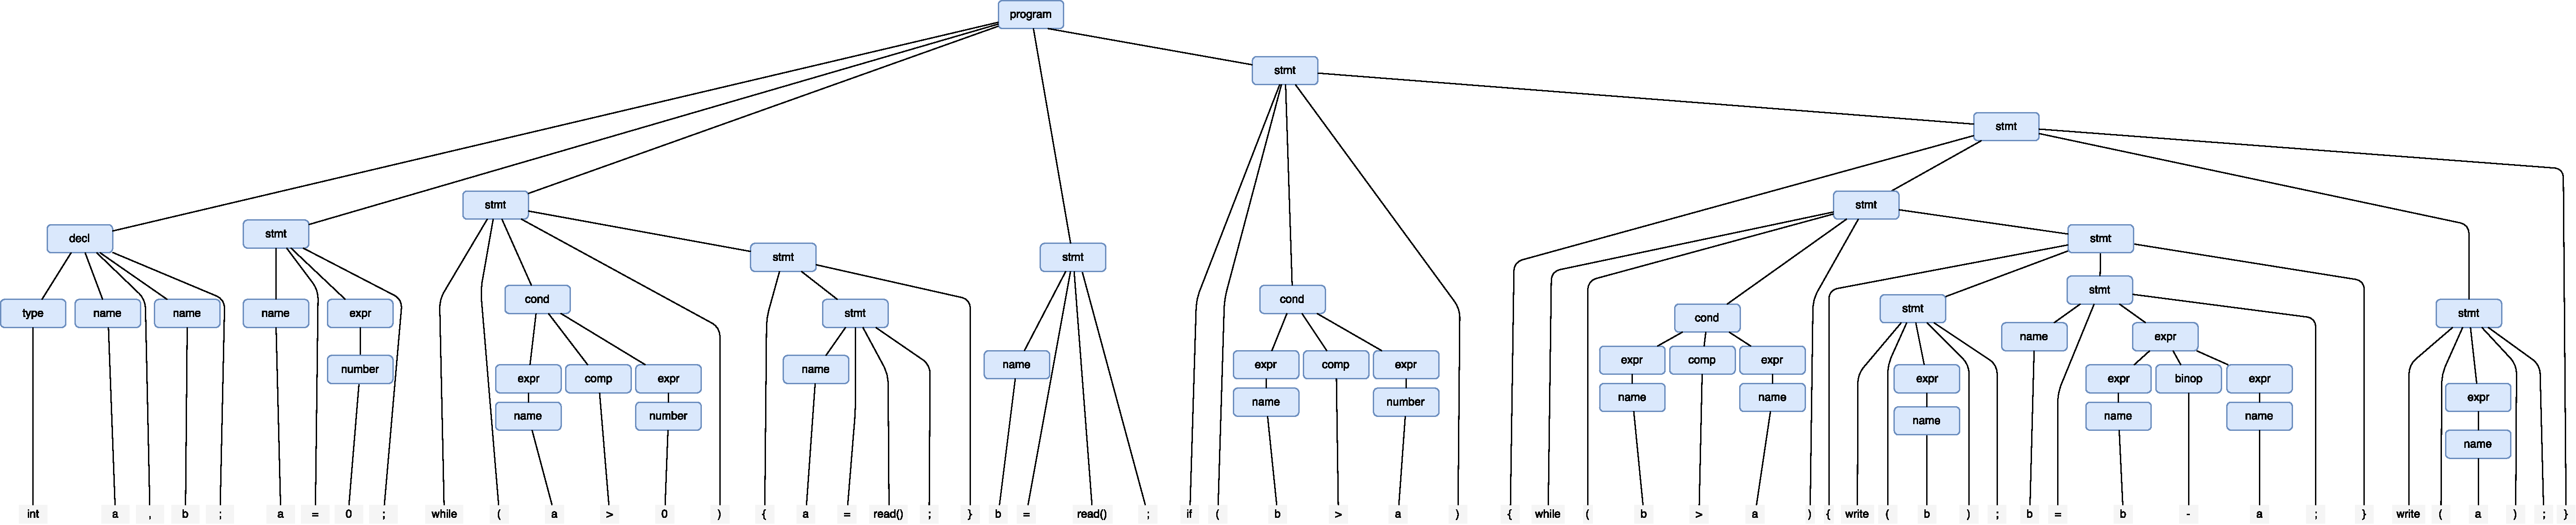
\includegraphics[width=\textwidth, height=\textheight, keepaspectratio]{syntax}
	\caption{Syntaxbaum}
\end{sidewaysfigure}
\begin{figure}[htpb]
	\centering
	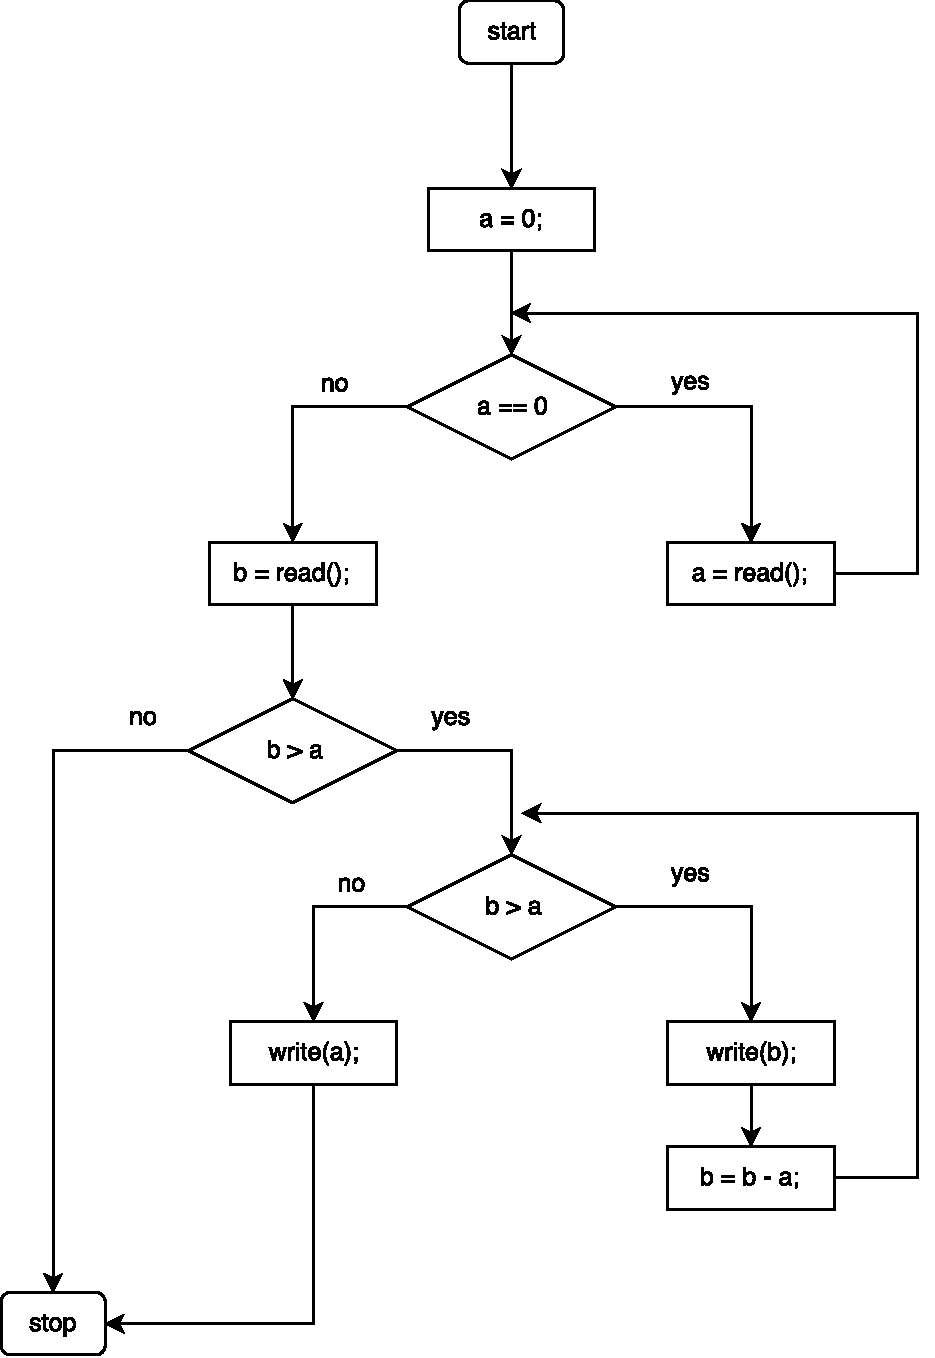
\includegraphics[width=\textwidth, height=\textheight, keepaspectratio]{kontrollfluss}
	\caption{Kontrollflussdiagramm}
\end{figure}
\end{document}